\documentclass[a4paper 14pt]{extarticle}
\usepackage[utf8]{vietnam}
\usepackage{amsmath}
\usepackage{amsthm}
\usepackage{amsfonts}
\usepackage{amssymb}
\usepackage{float}
\usepackage[document]{ragged2e}
%for use of addmargin environment
\usepackage{scrextend}

\usepackage[margin = 1in]{geometry}
\usepackage{caption}
\captionsetup{belowskip=12pt,aboveskip=4pt}
\usepackage{graphicx}

\graphicspath{{images/}}

\begin{document}
	\begin{titlepage}
\begin{center}
	\large{\textbf{ĐẠI HỌC QUỐC GIA THÀNH PHỐ HỒ CHÍ MINH}}\\
	\large{\textbf{TRƯỜNG ĐẠI HỌC KHOA HỌC TỰ NHIÊN}}\\
	\large{\textbf{KHOA CÔNG NGHỆ THÔNG TIN}}\\
	\vfill
	\begin{figure}[H]
		\centerline{
\includegraphics[scale = 0.5]{logo}}
	\end{figure}

	\Large{\textbf{Khai thác dữ liệu và ứng dụng}}\\
	\Large{\textbf{BT03: Phân lớp dữ liệu}}\\

\end{center}
	\vfill
\begin{flushright}
	
	\begin{tabular}{l l l}
		GVLT: &Thầy Lê Hoài Bắc\\
		&\\
		GVTH: &Thầy Nguyễn Tiến Huy\\
		&\\
		Sv: &Nguyễn Phan Mạnh Hùng & 1312727\\
		&La Ngọc Thùy An & 1312716\\
	\end{tabular}
\end{flushright}


\end{titlepage}

	\pagebreak
	
	\section{Câu 1}
		\subsection{Câu a}
			\underline{\textbf{Câu hỏi:}} Tại sao phân lớp Bayes (Bayesian Classification) được gọi là "naive" (ngây thơ)?\\
			\underline{\textbf{Trả lời:}} Phân lớp Bayes được gọi là "naive" do việc giả định về giá trị của một thuộc tính là độc lập so với giá trị của các thuộc tính khác.
		\subsection{Câu b}
			\underline{\textbf{Câu hỏi:}} Tại sao cần có bước tỉa nhánh (tree pruning) trong cây quyết định?\\
			\underline{\textbf{Trả lời:}} Trước hết ta cần biết rằng dữ liệu thực tế luôn tồn tại những dữ liệu nhiễu (bất thường), do đó nếu như cây càng chi tiết và cố gắng fit mọi bộ dữ liệu thì sẽ dễ dẫn tới trường hợp overfitting. Do đó, bước tỉa nhánh nhằm loại bỏ những nhánh nhỏ lẻ (mang ít giá trị trong việc phân lớp dữ liệu) mà vẫn giữ được tính tổng quát của cây và không làm tăng sai số trên dữ liệu thực tế.
		\subsection{Câu c}
			\underline{\textbf{Câu hỏi:}} Các phương pháp như Decision tree, Bayesian, neural network được gọi là eager classification; ngược lại các phương pháp như kNN được gọi là lazy classification. So sánh ưu nhược điểm của hai nhóm phương pháp này.\\
			\underline{\textbf{Trả lời:}} \\
			\begin{tabular}{p{3in} | p{3in}}
				Eager classification & Lazy classification\\
				\hline
				\multicolumn{2}{c}{Ưu điểm}\\
				Không gian lưu trữ nhỏ.&Không bị mất thông tin do lưu trữ toàn bộ dữ liệu.\\
				Mang tính tổng quát.&Giai đoạn train nhanh (hoặc gần như không có như trong kNN).\\
				Ít bị ảnh hưởng bởi nhiễu.&Tính toán được các hàm phức tạp.\\
				Truy vấn nhanh.&\\
				\hline
				\multicolumn{2}{c}{Nhược điểm}\\
				Gặp khó khăn trong việc xây dựng các hàm phức tạp, và khó đưa ra các xấp xỉ tốt cục bộ của hàm mục tiêu.&Không gian lưu trữ lớn, do phải lưu toàn bộ dữ liệu.\\
				Thông tin không bảo toàn do thường chỉ lưu trữ hàm hypothesis.&Dễ bị các điểm nhiễu ảnh hưởng.\\
				&Truy vấn chậm, do thường phải duyệt toàn bộ tập dữ liệu.\\
			\end{tabular}
	\section{Câu 2}
		Dữ liệu\\
		\begin{tabular}{c | c}
			X & Y\\
			Giữa kỳ&Cuối kỳ\\
			\hline
			75 & 84\\
			50 & 62\\
			80 & 77\\
			74 & 79\\
			94 & 90\\
			86 & 75\\
			59 & 50\\
			84 & 78\\
			61 & 75\\
			33 & 45\\
			88 & 85\\
			81 & 90\\
		\end{tabular}
		\subsection{Câu a}
			\underline{\textbf{Câu hỏi:}} Giữa điểm giữa kỳ (x) và điểm cuối kỳ (y) có mối quan hệ tuyến tính không?\\
			\underline{\textbf{Trả lời:}}\\
			\begin{figure}[H]
				\includegraphics[scale = 0.3]{datapoint}
				\caption{Biểu đồ biểu diễn các điểm dữ liệu}
			\end{figure}
			Dựa vào biểu đồ trên, ta nhận thấy điểm dữ liệu biểu diễn điểm giữa kì và cuối kì dường như dao động xung quanh 1 đường thẳng.\\
			Dựa vào đó, ta đưa ra dự đoán rằng giữa điểm giữa kỳ (x) và điểm cuối kỳ (y) có mối quan hệ tuyến tính.
		\subsection{Câu b}
			\underline{\textbf{Câu hỏi:}} Dùng phương pháp method of least squares để tìm phương trình dự đoán điểm cuối kỳ dựa vào điểm giữa kỳ.\\
			\underline{\textbf{Trả lời:}}\\
			\begin{tabular}{p{2in} l}
				Xét phương trình: & $h(x) = \theta_0 + \theta_1x$\\
				Hàm chi phi dựa vào method of least squares: & $J(X) = \frac{1}{n}\sum\limits_{i = 1}^{n}(h(x_i) - y_i)^2$\\ 
				n&số bộ dữ liệu, hay số cặp điểm giữa kì và cuối kì.\\
				$x_i$&điểm giữa kì thứ i\\
				$y_i$&điểm cuối kì tương ứng thứ i\\
			\end{tabular}\\
			Ta cần tìm $\theta =$\( \begin{bmatrix} \theta_0\\ \theta_1\\	\end{bmatrix}\), sao cho $J(X)$ là nhỏ nhất.\\
			Sử dụng Normal equation, ta tìm được $\theta$ theo công thức sau:\\
			\begin{equation}
				\theta = (A^TA)^{-1}A^TY
			\end{equation}\\
		
			Với A = [$alpha$ X], trong đó $\alpha^T = (1,1,...,1) \in R^n$, và $X^T = (x_1,x_2,...,x_n)$\\
			Ta giải được $\theta$ = \(\begin{bmatrix} 23.2841\\0.7059 \end{bmatrix}\).\\
			Vậy $h(x) = 23.2841 + 0.7059x$
			Dựa vào kết quả tìm được, ta có được đường thẳng sau:\\
			\begin{figure}[H]
				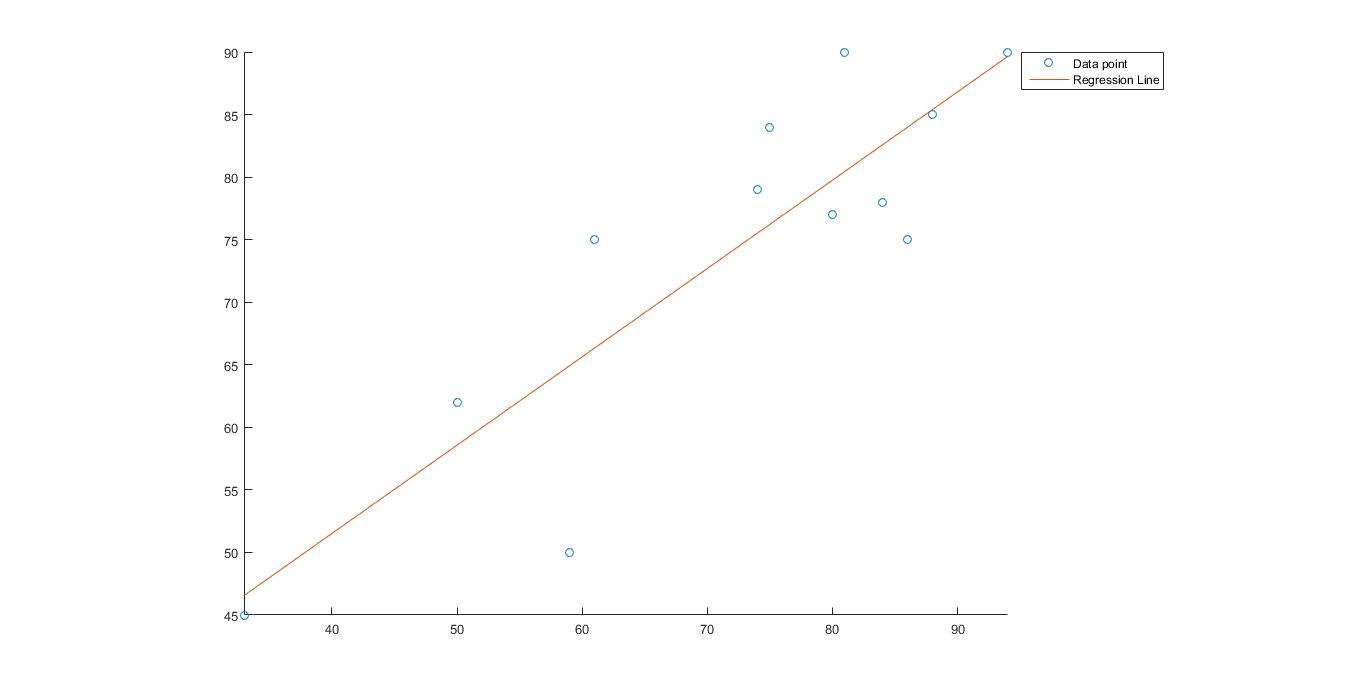
\includegraphics[scale = 0.3]{regression}
				\caption{Biểu đồ biểu diễn phương trình dự đoán điểm cuối kì theo điểm giữa kì}
			\end{figure}
		\subsection{Câu c}
			Với phương trình tìm được, ta dễ dàng tính $h(79) = 79.0490$ 
		\subsection{Source}
			Nhóm em cũng đã viết chương trình câu 2 bằng matlab.\\
			Source được lưu trong thư mục MethodOfLeastSquare trong Program nếu Thầy cần kiểm tra.
	\section{Câu 3}
		Sources được lưu trong thư mục KNN trong thư mục Program.\\
		Trước khi chạy chương trình, xin Thầy đọc qua file README.txt để nắm được input's format.
	\section{Đánh giá công việc}
	Bảng phân công nhiệm vụ\\
	\begin{tabular}{c | p{4in}}
		Nhiệm vụ & Thành viên \\
		\hline
		Câu 1&Mạnh Hùng\\
		Câu 2&2 thành viên cùng thảo luận, làm cá nhân và tổng hợp, so khớp kết quả.\\
		Câu 3&Thùy An
	\end{tabular}
\end{document}